% ====== TAREA 3 MATEMATICAS APLICADAS ======
\documentclass{article}
\usepackage[utf8]{inputenc}
\usepackage[spanish]{babel}
\usepackage{amsmath, amsfonts, amssymb}
% \usepackage{ tipa }
\usepackage{graphicx}
\usepackage[usenames]{color}
\usepackage[text={20cm,25cm},centering,top=1.5cm,bottom=1.5cm,letterpaper,showframe=false]{geometry}
\renewcommand{\baselinestretch}{1.5}
\parindent  = 0mm
\parskip    = 4mm
\definecolor{azul}{RGB}{10,80,190}
\definecolor{negro}{RGB}{0,0,0}
\definecolor{rojo}{RGB}{190,80,10}
\definecolor{verde}{RGB}{0,120,50}

\begin{document}
    \title{Tarea-Examen 3}
    \author{Careaga Carrillo Juan Manuel\\
            Quiróz Castañeda Edgar\\
            Soto Corderi Sandra del Mar}
    \date{Viernes 7 de diciembre de 2018}
    \maketitle
    \begin{enumerate}

        % Ejercicio 1
        \item {
            Demostrar que

            \begin{enumerate}
            \item{
				$\nabla \times (f \mathbf{F}) = f \nabla \times \mathbf{F} + \nabla f \times \mathbf{F}$

			\color{azul}
            % Respuesta


            }

            \item{
            	$\nabla \times (\nabla \times \mathbf{F}) = \nabla (\nabla \cdot \mathbf{F}) - \nabla^2 \mathbf{F}$

           \color{azul}
            % Respuesta

            }
            \end{enumerate}
	    }

        % Ejercicio 2
        \item {
            Determinar el rotacional y la divergencia de los campos

            \begin{enumerate}
            \item{
				$\mathbf{F} (x,y,z) = (0,\cos xz,\sin xy)$

			\color{azul}
            % Respuesta
            }

            \item{
            	$\mathbf{F} (x,y,z) = (\frac{x}{x^2 + y^2 + z^2}, \frac{y}{x^2 + y^2 + z^2}, \frac{z}{x^2 + y^2 + z^2})$

           \color{azul}
            % Respuesta

            }
            \end{enumerate}
        }

        % Ejercicio 3
        \item {
            Determinar si $\mathbf{F}$ es campo vectorial conservativo y en su caso encuentre el campo escalar $f$

            \begin{enumerate}
            \item{
				$\mathbf{F} (x,y) = (2x\cos y - y\cos x, -x^2\sin y -\sin x)$

			\color{azul}
            % Respuesta


            }

            \item{
            	$\mathbf{F} (x,y,z) = (2xy, x^2 + 2yz, y^2)$

           \color{azul}
            % Respuesta

            }
            \end{enumerate}
        }

        % Ejercicio 4
        \item {
           Calcular $\displaystyle\int_{C} \mathbf{F} \cdot d \mathbf{l}$

            \begin{enumerate}
            \item{
                $\mathbf{F} (x,y,z) = (\sin x,\cos y,xz)$ y la parametrización
                $\sigma (t) = (t^3,-t^2,t)$ con $0\leq t\leq 1$
                \color{azul}
                % Respuesta
                \begin{align*}
                    \int_{C}{\mathbf{F} \cdot d \mathbf{l}}
                    &= \int_{0}^{1}{
                        \left(\sen{t^3}, \cos{(-t^2)}, t^4\right)
                        \cdot\left(3t^2, -2t, 1 \right)
                    \,dt}\\
                    &= \int_{0}^{1}{\left(
                        3t^2\sen{t^3}-2t\cos{t^2}+t^4
                    \right)\,dt}\\
                    &= \left[
                        -\cos{t^3}-\sen{t^2}+\frac{t^5}{5}
                        \right]_{0}^{1}\\
                    &= 1-\cos{(1)}
                \end{align*}
            }
            \item{
                $\mathbf{F} (x,y) = (x-y,xy)$ y $C$ el arco de círculo
                $x^2 + y^2 = 4$ que se recorre en sentido antihorario de $(2,0)$
                a $(0,-2)$

                \color{azul}
                % Respuesta
                Primero demos una parametrización adecuada para $C=\vec{\sigma}
                (t)$, tomando en cuenta que se trata de una circunferencia con
                centro en el origen del plano y de radio $r=\sqrt{4}=2$.

                Se podría utilizar la siguiente parametrización
                \[
                    \vec{\sigma}_1(t)=(2\cos{t}, 2\sen{t});\hspace{10pt}
                    \frac{3\pi}{2}\leq t\leq 2\pi
                \]
                pero los límites de la integral se volverían complicados, por
                lo que podemos ajustar la parametrización a la siguiente
                \[
                    \vec{\sigma}(t)=(2\sen{t},-2\cos{t}); \hspace{10pt}
                    0\leq t\leq\frac{\pi}{2}
                \]
                Entonces
                \begin{align*}
                    \int_{C}{\mathbf{F} \cdot d \mathbf{l}}
                    &= \int_{0}^{\frac{\pi}{2}}{
                        \left(
                            2\sen{t}+2\cos{t}, -4\sen{t}\cos{t}
                        \right)\cdot
                        \left(
                            2\cos{t}, 2\sen{t}
                        \right)
                    dt}\\[0.3cm]
                    &= \int_{0}^{\frac{\pi}{2}}{
                        \left(
                            4\sen{t}\cos{t}+4\cos^2{t}-8\sen^2{t}\cos{t}
                        \right)
                    dt}\\[0.3cm]
                    &= 4\int_{0}^{\frac{\pi}{2}}{\sen{t}\cos{t}\,dt}
                    +4\int_{0}^{\frac{\pi}{2}}{\cos^2{t}\,dt}
                    -8\int_{0}^{\frac{\pi}{2}}{\sen^2{t}\cos{t}\,dt}\\[0.3cm]
                    &= (4)\frac{1}{2}\sen^2{t}\Big|_{0}^{\frac{\pi}{2}}
                    +4\int_{0}^{\frac{\pi}{2}}{\left(
                        \frac{1}{2}+\frac{1}{2}\cos{2t}
                    \right)dt}
                    -(8)\frac{1}{3}\sen^3{t}\Big|_{0}^{\frac{\pi}{2}}\\[0.3cm]
                    &= \left[
                        2\sen^2{t}+2t+\sen{2t}-\frac{8}{3}\sen^3{t}
                    \right]_{0}^{\frac{\pi}{2}}\\[0.3cm]
                    &= 2 + \pi + 0 - \frac{8}{3}\\
                    &= \pi - \frac{2}{3}
                \end{align*}
            }
            \end{enumerate}
        }

        % Ejercicio 5
        \item {
            Calcular $\displaystyle\iint_{S} f dS$

            \begin{enumerate}
            \item{
                $f(x,y,z) = x^2y + z^2$ y $S$ la parte del cilindro
                $x^2 + y^2 = 9$ que está entre los planos $z=0$ y $z=2$

                \color{azul}
                % Respuesta
                La proyección de $S$ sobre el plano $xz$ es un rectángulo con
                $x\in [-3,3]$ y $z\in [0,2]$ como se muestra en la figura
                \begin{center}
                    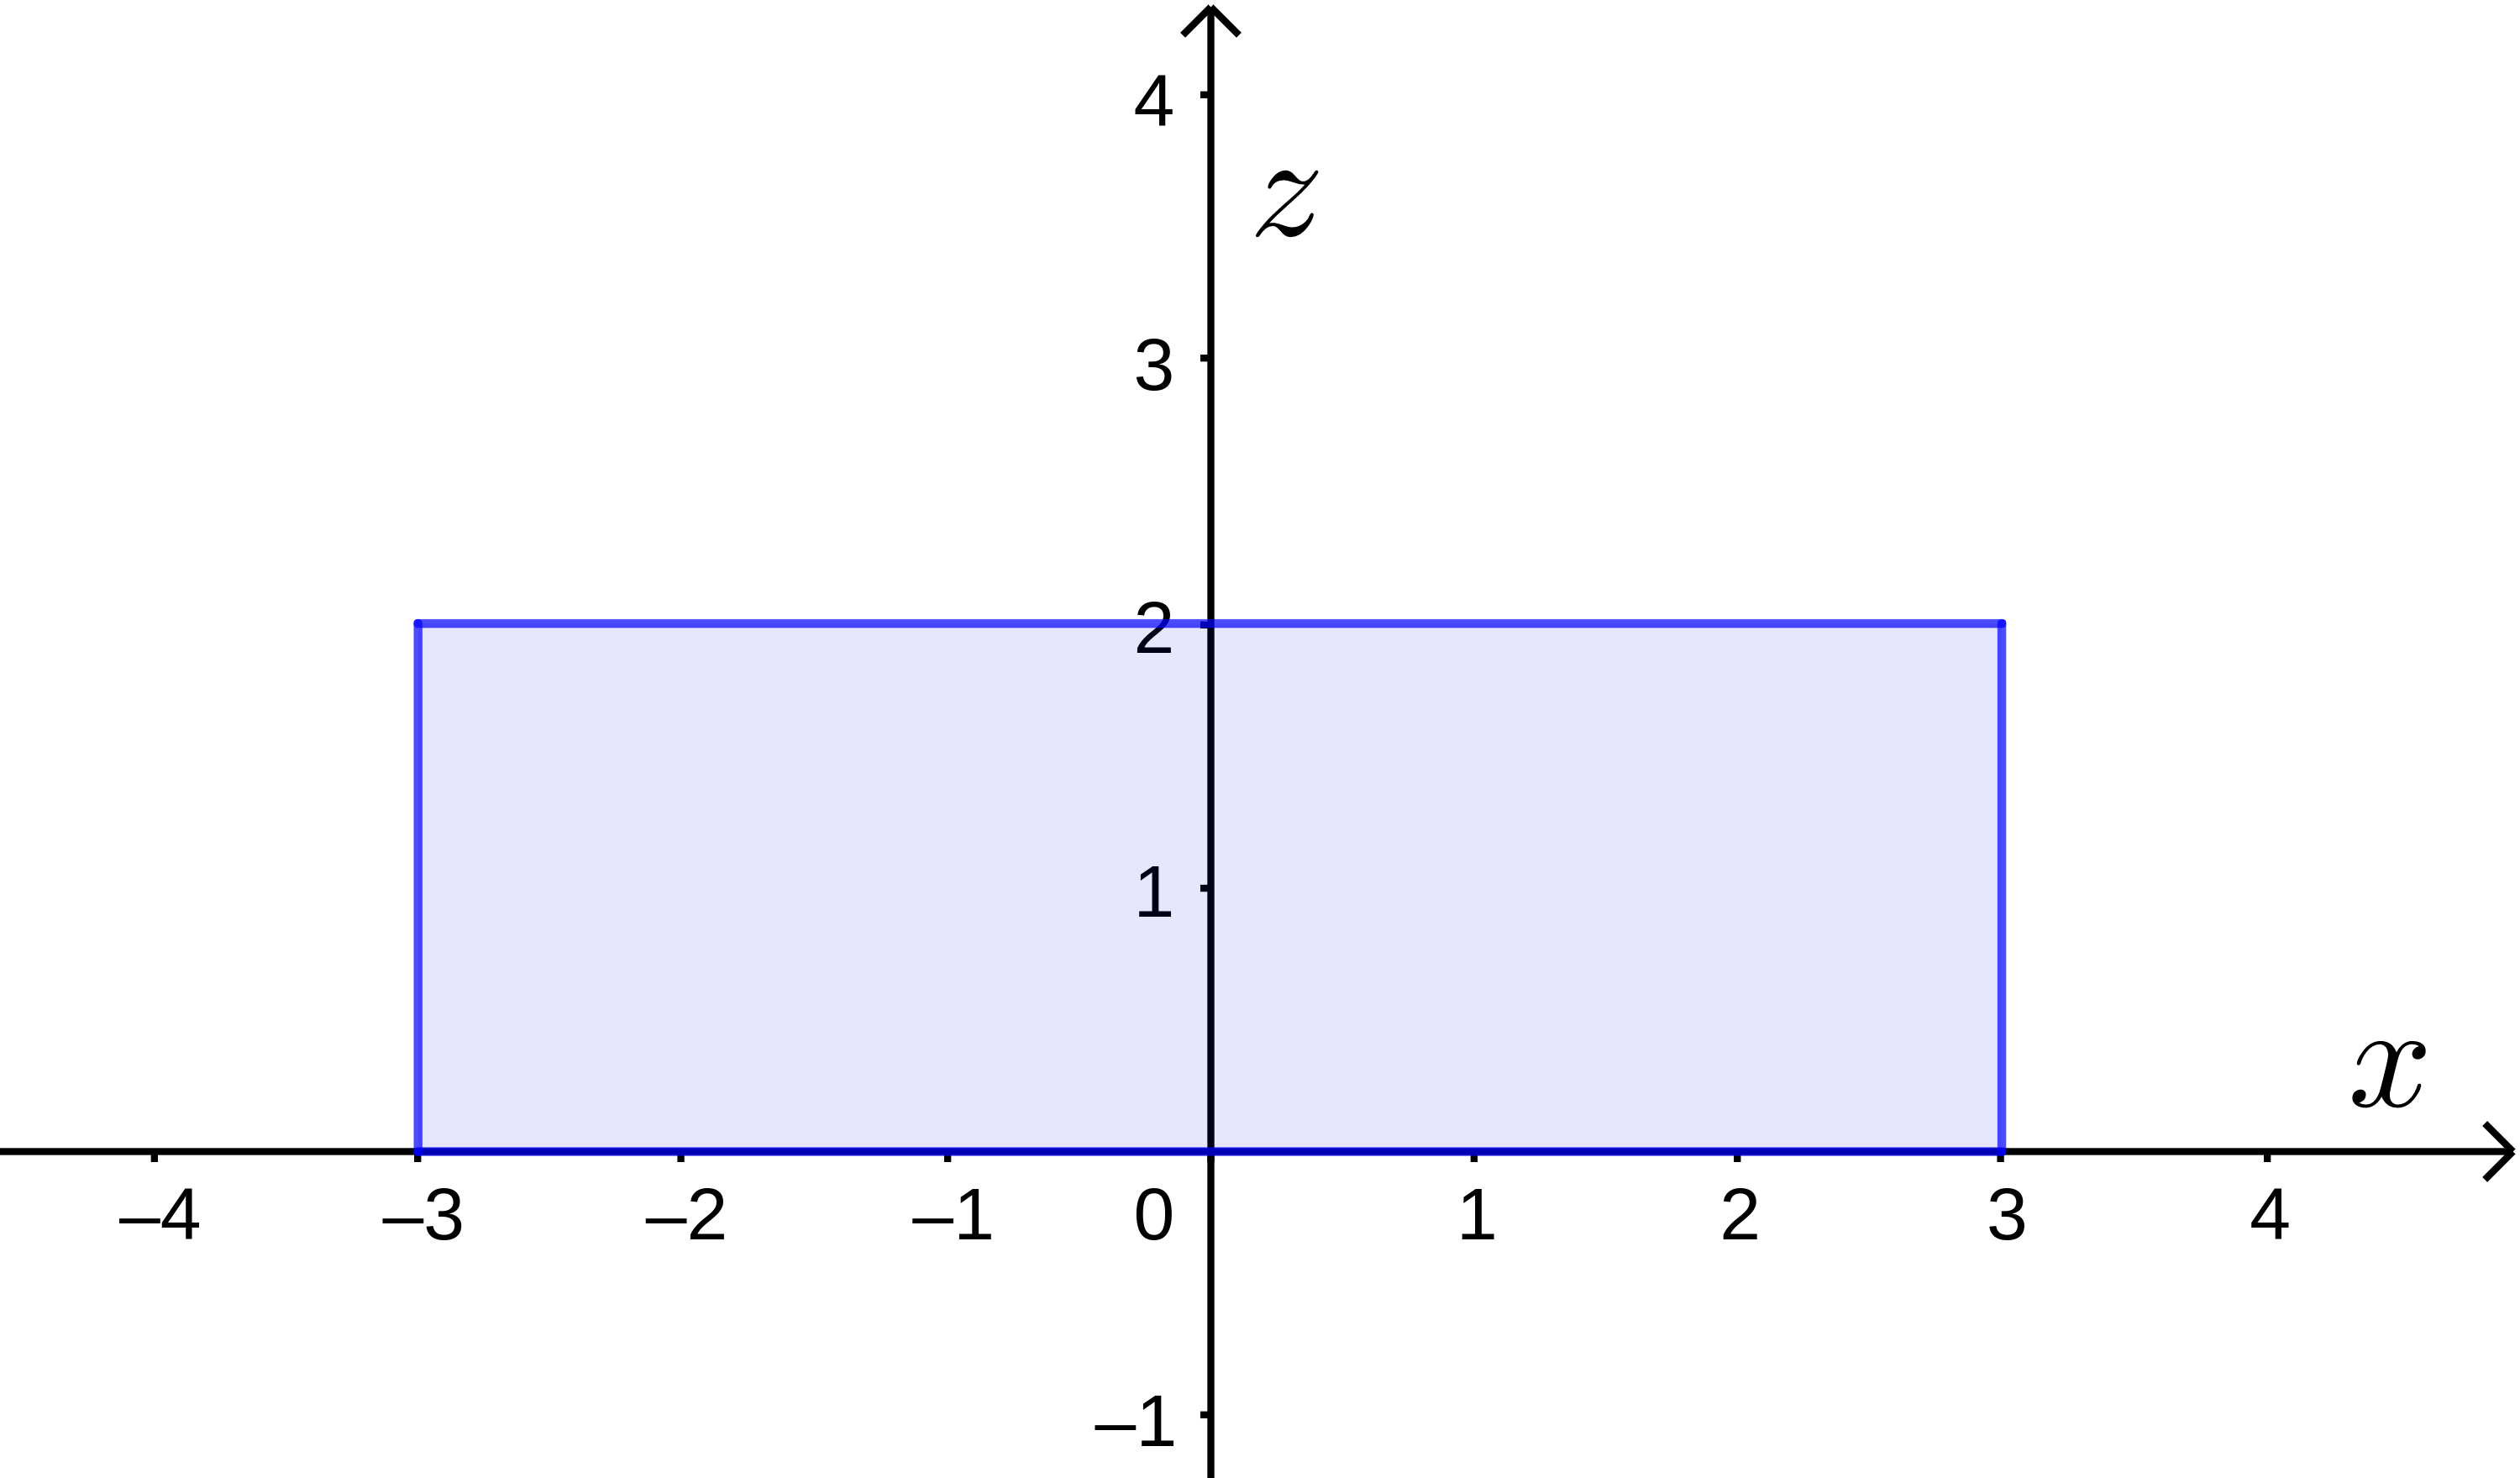
\includegraphics[width=6cm]{img/5a.png}
                \end{center}
                Escribimos la ecuación para $y=g(x,z)=\sqrt{9-x^2}$, entonces
                $\displaystyle g_x(x,z)=\frac{x}{\sqrt{9-x^2}}$ y
                $\displaystyle g_z(x,z)=0$

                Aplicando el teorema para convertir la integral de superficie
                en una integral doble
                \[
                    \displaystyle \iint_{S}{f(x,y,z)\,dS}
                    =\iint_{D}{
                        f(x,g(x,z), z)
                        \sqrt{\left[g_x(x,z)\right]^2+\left[g_z(x,z)\right]^2+1}
                    \,dA}
                \]
                Entonces tendremos que
                \begin{align*}
                    \iint_{S}{f(x,y,z)\,dS}
                    &= \iint_{D}{\left(
                        x^2 \sqrt{9-x^2}+z^2
                    \right)
                    \sqrt{
                        \frac{x^2}{9-x^2}+1
                    }
                    \,dA}\\[.3cm]
                    &= \int_{-3}^{3}{
                        \int_{0}^{2}{
                            \left(
                                3x^2+\frac{3z^2}{\sqrt{9-x^2}}
                            \right)
                        \,dz}
                    \,dx}\\[.3cm]
                    &= \int_{-3}^{3}{
                        \left[
                            3x^2z+\frac{z^3}{\sqrt{9-x^2}}
                        \right]_{0}^{2}
                    \,dx}\\[.3cm]
                    &= \int_{-3}^{3}{
                        \left(
                            6x^2+\frac{8}{\sqrt{9-x^2}}
                        \right)
                    \,dx}\\[.3cm]
                    &= \left[
                        2x^3+8\sen^{-1}{\left(\frac{x}{3}\right)}
                    \right]_{-3}^{3}\\
                    &= 108 + 8\pi
                \end{align*}
            }

            \item{
                $f(x,y,z) = x^2yz$ y $S$ la parte del plano $z = 1 + 2x + 3y$
                que está arriba del rectángulo $[0,3] \times [0,2]$

                \color{azul}
                % Respuesta
                Se entiende que la región $D = [0,3] \times [0,2]$, es la
                proyección acotada del plano $S$ sobre el plano $xy$, o sea que
                $x\in[0,3]$ e $y\in[0,2]$.

                Sea $z=g(x,y)$, entonces $g_x(x,y)=2$ y $g_y(x,y)=3$. Ahora
                aplicamos el teorema
                \begin{align*}
                    \iint_{S}{f(x,y,z)\,dS}
                    &= \iint_{D}{
                        f(x,y,g(x,y))
                        \sqrt{
                            \left[g_x(x,y)\right]^2+\left[g_y(x,y)\right]^2+1
                        }\,dA}\\[.2cm]
                    &= \int_{0}^{2}{
                        \int_{0}^{3}{
                            x^2y\left(1+2x+3y\right)
                            \sqrt{4+9+1}
                        \,dx}
                    \,dy}\\[.2cm]
                    &= \sqrt{14}\int_{0}^{2}{
                        \int_{0}^{3}{
                            \left(x^2y+2x^3y+3x^2y^2\right)
                        \,dx}
                    \,dy}\\[.2cm]
                    &= \sqrt{14}\int_{0}^{2}{
                        \left[
                            \frac{x^3y}{3}+\frac{x^4y}{2}+x^3y^2
                        \right]_{0}^{3}
                        \,dy}\\[.2cm]
                    &= \sqrt{14}\int_{0}^{2}{
                        \left(
                            9y+\frac{81}{2}y+27y^2
                        \right)
                    \,dy}\\[.2cm]
                    &=\sqrt{14}\left[
                        \frac{99}{4}y^2+9y^3
                    \right]_0^2\\
                    &= 71\sqrt{14}
                \end{align*}
            }
            \end{enumerate}


	    }

        % Ejercicio 6
        \item {
           Calcular $\displaystyle\iint_{S} \mathbf{F} \cdot d \mathbf{S}$

            \begin{enumerate}
            \item{
                $\mathbf{F} (x,y,z) = (0,y,-z)$ y $S$ consiste en el paraoloide
                $y = x^2 + z^2$, $0 \leq y \leq 1$, y el disco
                $x^2 + z^2 \leq 1$, $y = 1$

			\color{azul}
            % Respuesta


            }

            \item{
            	$\mathbf{F} (x,y) = (xze^y,-xze^y,z)$ y $S$ la parte del plano $x + y+ z = 1$ en el primer octante con orientación hacia arriba

           \color{azul}
            % Respuesta

            }
            \end{enumerate}


        }

        % Ejercicio 7
        \item {
            Usar el teorema de Stokes para evaluar $\displaystyle\iint_{S} \nabla \times \mathbf{F} \cdot d\mathbf{S}$, donde $\mathbf{F}(x,y,z) =(x^2y^3z,\sin(xyz),xyz)$ y $S$ es la parte del cono $y^2 = x^2 + z^2$ que está entre los planos $y = 0$ y $y = 3$ orientada en dirección positiva del eje Y.

            \color{azul}
            % Respuesta

        }

        % Ejercicio 8
        \item {
            Usar el teorema de Gauss para evaluar $\displaystyle\iint_{S} \mathbf{F} \cdot d\mathbf{S}$, con $\mathbf{F}(x,y,z) = (x^3y,-x^2y^2,-x^2yz)$ y $S$ la superficie cerrada definida por el hiperboloide $x^2 + y^2 - z^2 = 1$ y los planos $z = -2$ y $z = 2$

            \color{azul}
            % Respuesta

        }

         % Ejercicio 9
        \item {
            Usar propiedades del rotacional para mostrar que
            \[
                \int_C {{\left(f \nabla g + g \nabla f\right)}\,d\mathbf{l}} = 0
            \]


            \color{azul}
            % Respuesta

        }
    \end{enumerate}
\end{document}
